\documentclass[12pt, a4paper]{article}

%%%%%% 	pacotes	%%%%%%%
\usepackage[utf8]{inputenc}
\usepackage[portuguese]{babel}
\usepackage[T1]{fontenc}
%\usepackage{fontspec} % habilita o comando /setmainfont{times new roman}
\usepackage{graphicx, wrapfig} % para importar imagens e para coloca-las ao lado do texto

\usepackage{amsmath, amsfonts, amssymb}

\usepackage{blindtext} % para gerar textos com o comando \blindtext[1]

\usepackage[left=3cm,right=2cm,top=3cm,bottom=2cm]{geometry} % definindo as medidas das margens do papel

%%%%%%%	preambulo	%%%%%%
%\setmainfont{Times New Roman}
\setlength{\baselineskip}{1.5cm} %define a distancia/espaçamento entre linhas para ser 1.5 cm (o padrao da norma ABNT)
%\setlength{\parindent}{1.25cm} %define o recuo do paragrafo para ser 1.25cm (o padrao da norma ABNT)
\setlength{\parindent}{0cm}

\begin{document}
\pagestyle{empty}

\begin{wrapfigure}{L}{0.1\textwidth} % o parametro L: a posição da imagem em relação ao texto: a esquerda do texto. outros valores: l, r, i, o, R, O, I. Já o segundo parametro indica o quao perto o texto esta da imagem. Mudar apenas o valor numerico
\includegraphics[width=0.065\textheight]{logo ufpe.jpg}
%separando cada linha por multiplos de 1.5cm, o espaçamento padrão segundo as normas da ABNT.

\end{wrapfigure}

\noindent UNIVERSIDADE FEDERAL DE PERNAMBUCO\\CENTRO DE CIÊNCIAS EXATAS E DA NATUREZA\\DEPARTAMENTO DE MATEMÁTICA\\PRINCÍPIOS DE CONTAGEM - 2023.1\\PROFESSOR: WILLIKAT BEZERRA DE MELO\\TURMA: 2Z\\

\begin{flushleft}

MONITOR: JARDEL FELIPE CABRAL DOS SANTOS\\[1cm] 
\end{flushleft}

\begin{center} \textbf{ENCONTRO DE MONITORIA - 04/08/2023\\[1cm]}
\end{center}

\begin{center}
\textbf{PROBLEMAS}
\end{center}

\textbf{1. Tem-se 8 pontos sobre uma reta \(r\) e 11 pontos sobre uma reta \(r'\) paralela a \(r\). Quantos quadriláteros não-convexos com vértices em \(4\) desses \(19\) pontos existem?} \\

\textbf{2. Quantos são os anagramas da palavra SORRIR? Quantos deles tem a letra S no primeiro lugar ou a letra O no segundo lugar?} \\

\textbf{3. De quantos modos podemos dividir 16 pessoas em dois grupos de 4 pessoas e um grupo de 8 pessoas?} \\

\begin{center}
\textbf{RESOLUÇÃO}
\end{center}

\textbf{1.}

Um quadrilátero pode ser determinado a partir de \(4\) pontos (seus vértices) que não sejam colineares quando considerados três-a-três. A quantidade de maneiras de selecionar \(4\) dos \(19\) pontos das retas é \(C^{19}_{4} = 3876\). Porém, note que nem todo conjunto de quatro pontos contabilizado formará um quadrilátero. Se \(3\) dos quatros pontos estiverem na mesma reta, então não teremos um quadrilátero. A quantidade de maneiras escolher \(3\) pontos em uma reta e um ponto na outra reta é \[C^{8}_{3}\times C^{11}_{1} + C^{8}_{1}\times C^{11}_{3}=616+1320=1936\]O primeiro produto é a quantidade de maneiras que \(3\) pontos são escolhidos na reta \(r\) e \(1\) ponto é escolhido na reta \(r'\). Já o segundo produto é a quantidade de maneiras que \(1\) ponto é escolhido na reta \(r\) e \(3\) pontos são escolhidos na reta \(r'\).\\

Além disso, se os \(4\) pontos estão na mesma reta, também não teremos um quadrilátero. A quantidade de maneiras que isso acontece é \(C^{8}_{4} + C^{11}_{4} = 70 + 330=400 \). (Por quê?) \\

Desse modo,  a expressão \[C^{19}_{4} - [(C^{8}_{3}\times C^{11}_{1} + C^{8}_{1}\times C^{11}_{3}) + (C^{8}_{4} + C^{11}_{4})]=3876-(1936+400)=1540\] nos diz a quantidade de maneiras de selecionar \(4\) pontos que formam um quadrilátero. Porém, note que essa não é a resposta, já  que queremos que os quadriláteros formados sejam não-convexos. Para isso, é necessário analisar: dado \(4\) pontos que formam um quadrilátero, quantos quadriláteros não-convexos diferentes podemos formar?\\

A resposta dessa pergunta é: \(2\) quadriláteros não-convexos. Veja abaixo uma figura que contém todos os quadriláteros que podem ser formados a partir de \(4\) pontos fixos, porém arbitrários. 
\begin{center}
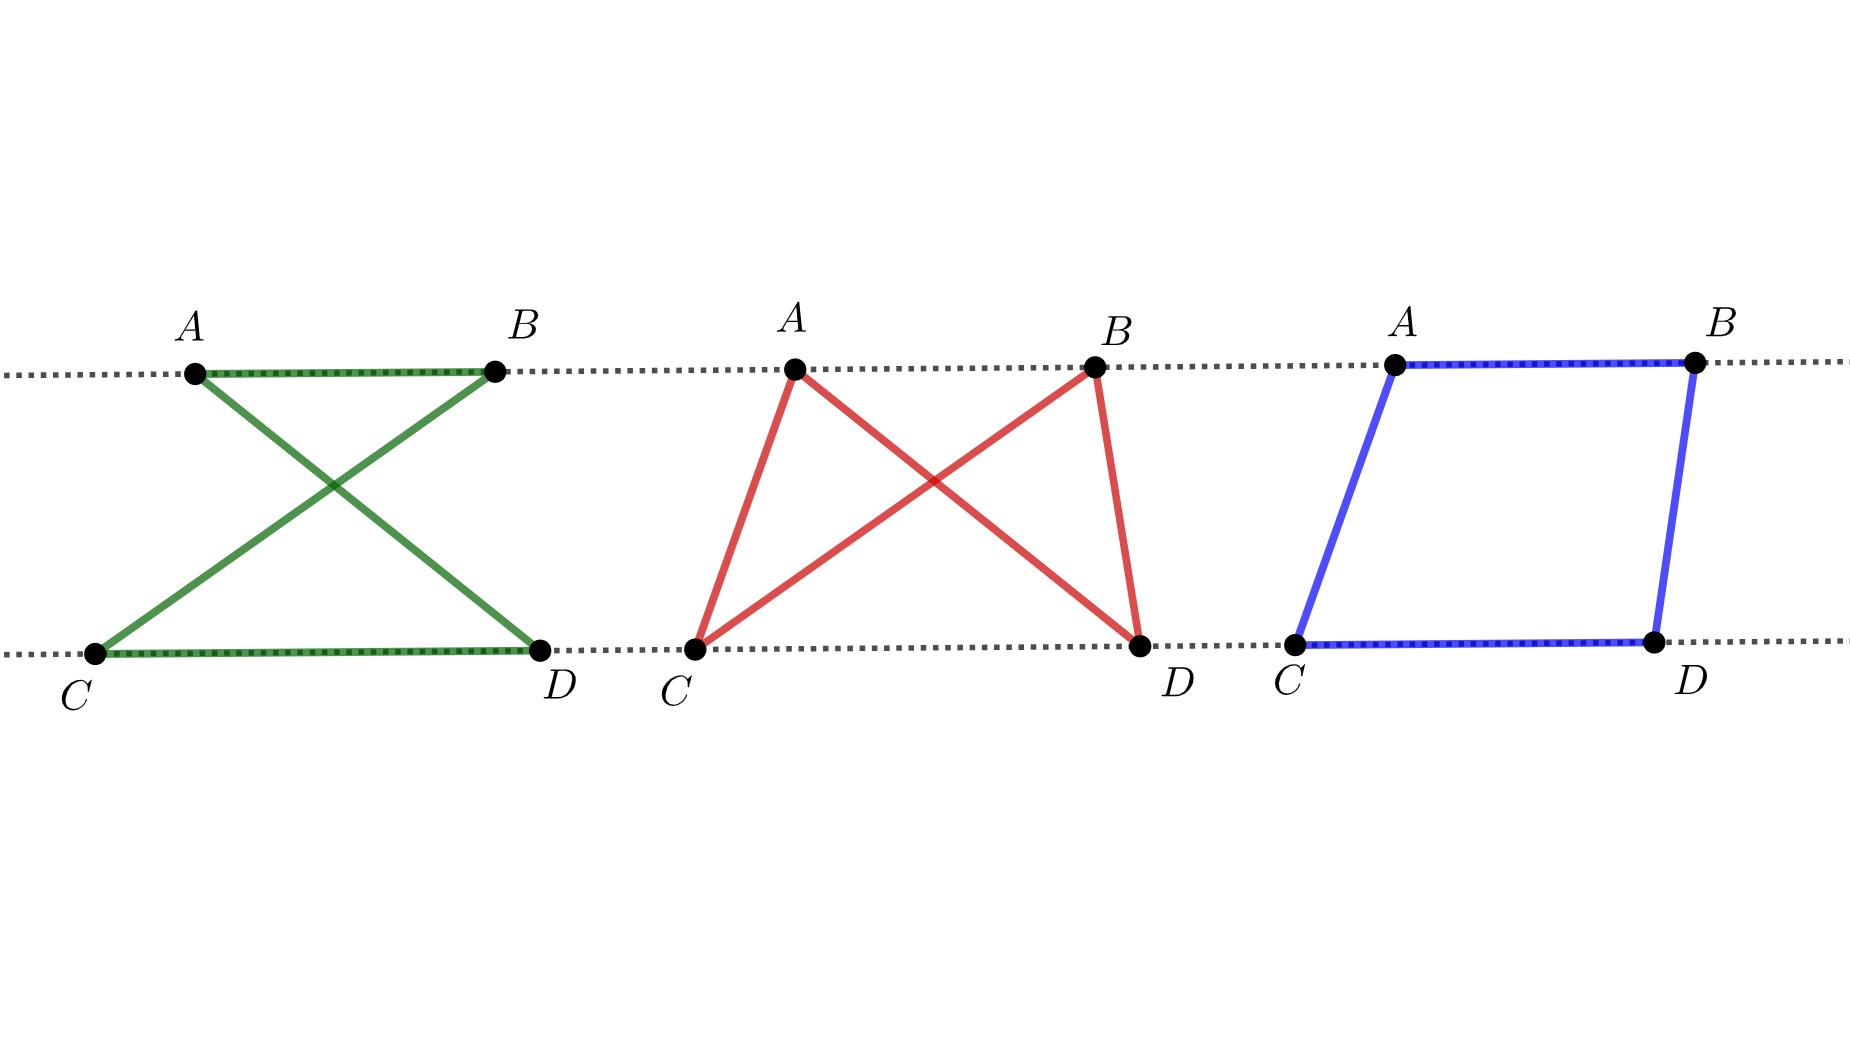
\includegraphics[scale=0.5]{fig_quad}
\end{center}
Sendo assim, cada conjunto de quatro pontos forma \(2\) quadriláteros não-convexos. Portanto, a quantidade de quadriláteros com a propriedade desejada é \(2 \cdot{1540} = 3080\). \\

\textbf{2.}

(a) Calculando quantos anagramas possui a palavra SORRIR: \\

Note que há repetição da letra R. Assim, utilizando a ideia de permutação com repetição, a quantidade de anagramas de SORRIR é: \[P_{(6;1,1,3,1)} = \dfrac{6!}{1! \times 1! \times 3! \times 1!} = 120\]

(b) Calculando quantos deles começam com S ou tem segunda letra sendo O: \\

Sejam \(A\) e \(B\) conjuntos tais que \(A\) é o conjunto de todos os anagramas de SORRIR que começam com S e \(B\) é o conjunto de todos os anagramas de SORRIR que tem segunda letra sendo O. Utilizaremos a notação \(|X|\) para indicar a quantidade de elementos de um conjunto \(X\). Desse modo, a resposta do item (b) será \(\left|A \cup B \right|\). \\

De modo geral, \(\left|A \cup B \right| = |A| + |B| - \left| A \cap B \right|\). Calcularemos abaixo \(|A|\), \(|B|\) e \(\left| A \cap B \right|\): \\

(i) Calculando \(|A|\):

Temos \(1\) maneira de escolher a posição do S (que seria a primeira letra do anagrama). Escolhida ela, podemos escolher as demais letras de \(P_{(5;1,3,1)} = 20\) maneiras. Assim, pelo princípio multiplicativo, temos \(1\cdot{20} = 20\) maneiras de formar um anagrama de SORRIR que comece com S. Portanto, \(|A| = 20\). \\

(ii) Calculando \(|B|\):

Temos \(1\) maneira de escolher a posição do O (que seria a segunda letra do anagrama). Escolhida ela, podemos escolher as demais letras de \(P_{(5;1,3,1)} = 20\) maneiras. Assim, de maneira análoga ao calculo de (i), temos \(|B| = 1\cdot{20} = 20\).\\

(iii) Calculando \(\left|A \cap B \right|\):

Temos \(1\) maneira de escolher a posição do S e do O (que seriam, respectivamente, a primeira e segunda letra do anagrama). Feito essa escolha, podemos escolher as demais letras de \(P_{(4;3,1)} = 4\) maneiras. Portanto, pelo princípio multiplicativo, temos \(\left|A \cap B \right|= 1\cdot{4} = 4\). \\

Desse modo, 
\[\left|A \cup B \right| = 20 + 20 - 4 = 36\]

\textbf{3.}

Podemos formar um grupo de \(8\) pessoas de \(C^{16}_{8}\) maneiras. Tendo sido formado um grupo de \(8\) pessoas, queremos formar dois grupos de \(4\) pessoas com as \(8\) pessoas que sobraram. Para o primeiro grupo, temos \(C^{8}_{4}\) maneiras de formá-lo. Já para o segundo grupo, temos \(C^{4}_{4}\) maneiras. \\

Pelo princípio multiplicativo, \(C^{8}_{4} \times C^{4}_{4}\) representa a quantidade de maneiras de formar os dois grupos de \(4\) pessoas de modo que seja possível distinguir cada grupo. Por exemplo: o primeiro grupo tem um nome diferente do segundo grupo. Desse modo, escolher os integrantes do primeiro grupo como sendo \(\{a,b,c,d\}\), e do segundo grupo como sendo \(\{e,f,g,h\}\), é contabilizado como sendo diferente de escolher os integrantes do primeiro grupo como sendo \(\{e,f,g,h\}\) e do segundo grupo como sendo \(\{a,b,c,d\}\). \\

Porém, para o problema, não há uma ordem ou hierarquia para os  grupos. Desse modo, cada caso é contando uma quantidade de vezes que é numericamente igual à quantidade de maneiras de permutar os dois grupos: \(P^2_2\). Portanto, a resposta deve ser \[\dfrac{C^{8}_{4} \times C^{4}_{4}}{P^2_2}\]
Daí, pelo princípio multiplicativo, a resposta do problema 3 será: \[C^{16}_{8} \times \left( \dfrac{C^{8}_{4} \times C^{4}_{4}}{P^2_2} \right) = \dfrac{16!}{2! \times 8! \times 4! \times 4!}\]

\end{document}